\documentclass[11pt]{article}
\usepackage{amsmath,amsfonts,amssymb,amsthm}

\usepackage{mathpazo}
\usepackage{fullpage}

\usepackage{tikz,ifthen}

\usepackage[colorlinks = true,
            linkcolor = blue,
            urlcolor  = blue]{hyperref}
\usepackage{color}

\theoremstyle{plain}
\newtheorem*{claim}{Claim}


%%%%%%%%%%%%%%%%%%%%%%%%%%%%%%%%%%%

\theoremstyle{plain}
\newtheorem*{theorem}{Theorem}

\theoremstyle{remark}
\newtheorem*{solution}{Solution}

\def\naturals{\mathbb{N}}
\def\integers{\mathbb{Z}}
\def\rationals{\mathbb{Q}}
\def\reals{\mathbb{R}}
\def\complex{\mathbb{C}}


\usepackage[most,breakable]{tcolorbox}
\renewenvironment{boxed}%
	{\begin{tcolorbox}[colback=white,colframe=gray!10,breakable,enhanced]}%
	{\end{tcolorbox}}

\begin{document}


\title{MATH 135 --- Fall 2021\\ Sample Proofs from Lecture 12}
\author{Mark Girard}

\maketitle

\section*{Chomp}
In a game of Chomp\footnote{You can find out more about Chomp on Wikipedia \url{https://en.wikipedia.org/wiki/Chomp}. You can play against a computer \href{https://www.math.ucla.edu/~tom/Games/chomp.html}{here}.}, players alternate turns taking cookies from a rectangular grid. At the beginning of the game, the grid is full of cookies. Below is an example of an initial board at the start of a game on a $4\times 5$ grid.

\begin{center}
 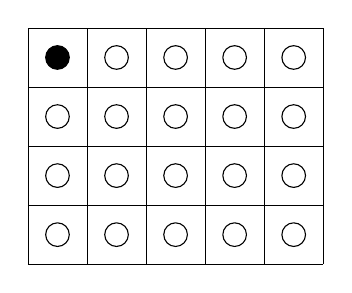
\begin{tikzpicture}[scale=0.75]
\draw[step=1cm,black,very thin] (0,0) grid (5,4);
\fill[black] (0.5,3.5) circle (0.2);
\foreach \x in {0,...,4}
    \foreach \y in {0,...,3}
        \draw (\x+.5,\y+.5) circle (.2);a
\end{tikzpicture}
\end{center}

\noindent Here are the rules of the game:
\begin{itemize}
 \item Two players alternate turns taking cookies off of the board. 
 \item On their turn, a player takes one of the cookies from the board and eats it, then also eats all other remaining cookies on the board that are below and to the right of that cookie. 
 \item The cookie in the top left corner is poison. Whoever eats the poison cookie loses this game! 
\end{itemize}

\noindent \textbf{Example game.} Below is a sequence of turns in an example game played between Alice (player one) and Bob (player two).
\begin{enumerate}
 \item Alice takes the cookie in row 3 and column 3, along with the other five cookies below and to the right.


\begin{center}
 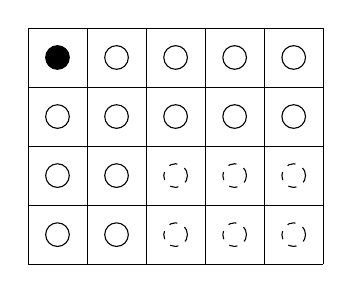
\begin{tikzpicture}[scale=0.75]
\draw[step=1cm,black,very thin] (0,0) grid (5,4);
\fill[black] (0.5,3.5) circle (0.2);
\foreach \x in {0,...,4}
    \foreach \y in {0,...,3}
        \ifthenelse{\x<2 \OR \y>1}
        {\draw (\x+.5,\y+.5) circle (.2);}
        {\draw[dashed] (\x+.5,\y+.5) circle (0.2);};
\end{tikzpicture}
\end{center}

\item In response, Bob takes the cookie in the top row and column 4, along with three other cookies in the top two rows.

\begin{center}
 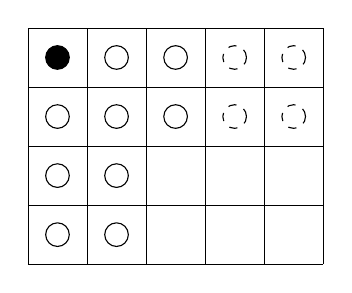
\begin{tikzpicture}[scale=0.75]
\draw[step=1cm,black,very thin] (0,0) grid (5,4);
\fill[black] (0.5,3.5) circle (0.2);
\foreach \x in {0,...,4}
    \foreach \y in {0,...,3}
        \ifthenelse{\x<2 \OR \y>1}
        {\ifthenelse{\x<3}
         {\draw (\x+.5,\y+.5) circle (.2);}
         {\draw[dashed] (\x+.5,\y+.5) circle (0.2);}
        }
        {};
\end{tikzpicture}
\end{center}

\item On Alice's second turn, she takes the farthest left cookie in the second row, along with all remaning cookies not in the top row.

\begin{center}
 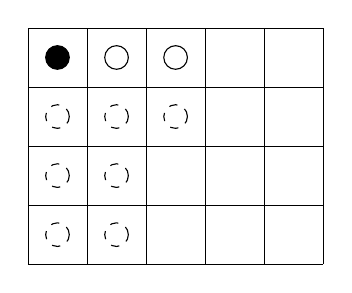
\begin{tikzpicture}[scale=0.75]
\draw[step=1cm,black,very thin] (0,0) grid (5,4);
\fill[black] (0.5,3.5) circle (0.2);
\foreach \x in {0,...,4}
    \foreach \y in {0,...,3}
        \ifthenelse{\x<2 \OR \y>1}
        {\ifthenelse{\x<3}
         {\ifthenelse{\y>2}
          {\draw (\x+.5,\y+.5) circle (.2);}
          {\draw[dashed] (\x+.5,\y+.5) circle (0.2);}
         }
        }
        {};
\end{tikzpicture}
\end{center}

\item On Bob's next turn, he takes the cookie immidiately to the right of the poison cookie along with the other remaining non-poison cookie.
\begin{center}
 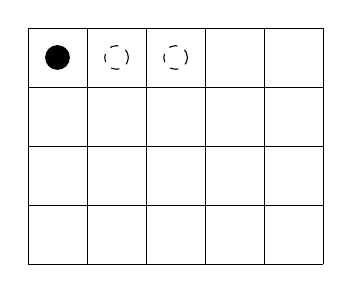
\begin{tikzpicture}[scale=0.75]
\draw[step=1cm,black,very thin] (0,0) grid (5,4);
\fill[black] (0.5,3.5) circle (0.2);
\foreach \x in {0,...,4}
    \foreach \y in {0,...,3}
        \ifthenelse{\x<2 \OR \y>1}
        {\ifthenelse{\x<3}
         {\ifthenelse{\y>2}
          {\ifthenelse{\x<1}
           {\draw (\x+.5,\y+.5) circle (.2);}
           {\draw[dashed] (\x+.5,\y+.5) circle (0.2);}
          }
         }
        }
        {};
\end{tikzpicture}
\end{center}
\item This leaves Alice with only one move---to take the poison cookie. Alice loses and \textbf{Bob wins}!

\end{enumerate}


\subsubsection*{Winning strategies for $2\times n$ Chomp}

Winning strategies for games of Chomp of arbitrary size are difficult to determine, but in the simple case of a $2\times n$ game it turns out that Alice always has a winning strategy. 

\begin{center}
 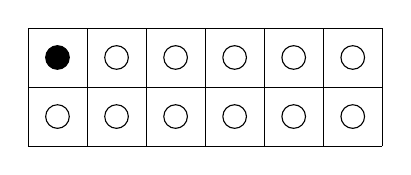
\begin{tikzpicture}[scale=0.75]
\draw[step=1cm,black,very thin] (0,0) grid (6,2);
\fill[black] (0.5,1.5) circle (0.2);
\foreach \x in {0,...,5}
    \foreach \y in {0,...,1}
        \draw (\x+.5,\y+.5) circle (.2);a
\end{tikzpicture}
\end{center}



\begin{tcolorbox}
\begin{claim}
 For all $n\in\naturals$, in a $2\times n$ game of Chomp, Alice has a winning strategy.
\end{claim}
\end{tcolorbox}


 
 
\begin{proof}
 To prove that Alice has a winning strategy, we first define an open sentence $P(n)$ for each $n\in\naturals$ as: 
 \begin{quotation}
  \noindent ``In a game of Chomp with only two rows, if it is Bob's turn and there are exactly $n$ cookies in the first row and $n-1$ cookies in the second row, then Alice can win the game regardles of what Bob does.''
 \end{quotation}
 We will first prove by induction that ``$\forall n\in\naturals,\, P(n)$'' is true.
 \begin{itemize}
  \item\underline{Base case:} Assume that $n=1$ and that it is Bob's turn and there is exactly 1 cookie in the top row and zero cookies in the bottom row. Then there is only one cookie remaining, which is the poison cookie. The game board must look like this:
  \begin{center}
 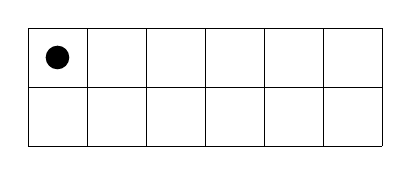
\begin{tikzpicture}[scale=0.75]
\draw[step=1cm,black,very thin] (0,0) grid (6,2);
\fill[black] (0.5,1.5) circle (0.2);
\end{tikzpicture}
\end{center}
  As it is Bob's turn, Bob must take the poison cookie and loses, so Alice wins. Thus, $P(1)$ is true.
\item\underline{\smash{Induction step}:} Let $k$ be an arbitrary natural number and suppose that $P(1),P(2),\dots$ and $P(k)$ are all true. That is, assume that
\[
 \forall m\in\naturals,\, m\leq k \implies P(m) \tag{Induction hypothesis}
\]
is true.
[We will now prove that $P(k+1)$ is true.] Suppose it is Bob's turn and there are exactly $k+1$ cookies in the top row and $k$ cookies in the bottom row. The game board must look something like this:
\begin{center}
 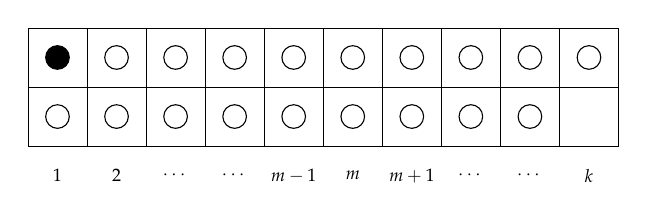
\begin{tikzpicture}[scale=0.75]
\draw[step=1cm,black,very thin] (0,0) grid (10,2);
\fill[black] (0.5,1.5) circle (0.2);
\foreach \x in {0,...,9}
    \foreach \y in {0,...,1}
        \ifthenelse{\x=9 \AND \y=0}
         {}
         {\draw (\x+.5,\y+.5) circle (.2);};
\draw(0.5,-.5) node[scale=.65]{$1$};
\draw(1.5,-.5) node[scale=.65]{$2$};
\draw(2.5,-.5) node[scale=.65]{$\cdots$};
\draw(3.5,-.5) node[scale=.65]{$\cdots$};
\draw(4.5,-.5) node[scale=.65]{$m-1$};
\draw(5.5,-.5) node[scale=.65]{$m$};
\draw(6.5,-.5) node[scale=.65]{$m+1$};
\draw(7.5,-.5) node[scale=.65]{$\cdots$};
\draw(8.5,-.5) node[scale=.65]{$\cdots$};
\draw(9.5,-.5) node[scale=.65]{$k$};
\end{tikzpicture}
\end{center}
Bob has two possible types of moves; he must either take a cookie from the top row or from the bottom row.
\begin{itemize}
    \item Case 1: Suppose Bob takes a cookie from the top row. He must then take a cookie in some column $m+1$, where $1\leq m\leq k$. In response, on Alice's next turn she can take the cookie in the second row in column $m$. The game board now looks like this:
\begin{center}
 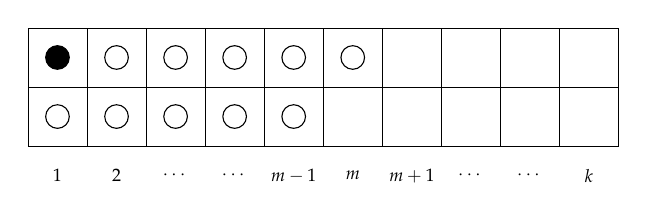
\begin{tikzpicture}[scale=0.75]
\draw[step=1cm,black,very thin] (0,0) grid (10,2);
\fill[black] (0.5,1.5) circle (0.2);
\foreach \x in {0,...,9}
    \foreach \y in {0,...,1}
        \ifthenelse{\x<6}
         {\ifthenelse{\y=1}
          {\draw (\x+.5,\y+.5) circle (.2);}
          {\ifthenelse{\y=0 \AND \x<5}
           {\draw (\x+.5,\y+.5) circle (.2);}
           {}
          }
        };
\draw(0.5,-.5) node[scale=.65]{$1$};
\draw(1.5,-.5) node[scale=.65]{$2$};
\draw(2.5,-.5) node[scale=.65]{$\cdots$};
\draw(3.5,-.5) node[scale=.65]{$\cdots$};
\draw(4.5,-.5) node[scale=.65]{$m-1$};
\draw(5.5,-.5) node[scale=.65]{$m$};
\draw(6.5,-.5) node[scale=.65]{$m+1$};
\draw(7.5,-.5) node[scale=.65]{$\cdots$};
\draw(8.5,-.5) node[scale=.65]{$\cdots$};
\draw(9.5,-.5) node[scale=.65]{$k$};
\end{tikzpicture}
\end{center}
It is now Bob's turn and there are $m$ cookies in the top row and $m-1$ cookies in the bottom row. Because $1\leq m\leq k$ and because it is assumed that $P(m)$ is true by the Induction Hypothesis, it follows that Alice can win regardless of what Bob does next. 
\item Case 2: Suppose Bob takes a cookie from the bottom row. He must then take a cookie in some column $m$, where $1\leq m\leq k$. In response, on Alice's next turn she can take the cookie in the top row in column $m+1$. The game board now looks like this:
\begin{center}
 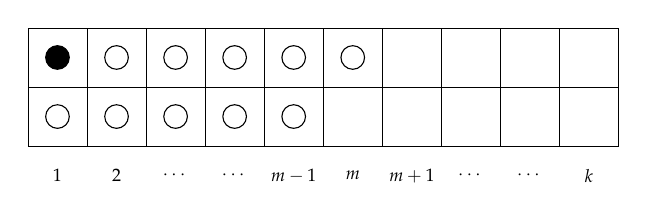
\begin{tikzpicture}[scale=0.75]
\draw[step=1cm,black,very thin] (0,0) grid (10,2);
\fill[black] (0.5,1.5) circle (0.2);
\foreach \x in {0,...,9}
    \foreach \y in {0,...,1}
        \ifthenelse{\x<6}
         {\ifthenelse{\y=1}
          {\draw (\x+.5,\y+.5) circle (.2);}
          {\ifthenelse{\y=0 \AND \x<5}
           {\draw (\x+.5,\y+.5) circle (.2);}
           {}
          }
        };
\draw(0.5,-.5) node[scale=.65]{$1$};
\draw(1.5,-.5) node[scale=.65]{$2$};
\draw(2.5,-.5) node[scale=.65]{$\cdots$};
\draw(3.5,-.5) node[scale=.65]{$\cdots$};
\draw(4.5,-.5) node[scale=.65]{$m-1$};
\draw(5.5,-.5) node[scale=.65]{$m$};
\draw(6.5,-.5) node[scale=.65]{$m+1$};
\draw(7.5,-.5) node[scale=.65]{$\cdots$};
\draw(8.5,-.5) node[scale=.65]{$\cdots$};
\draw(9.5,-.5) node[scale=.65]{$k$};
\end{tikzpicture}
\end{center}
It is now Bob's turn and there are $m$ cookies in the top row and $m-1$ cookies in the bottom row. Because $1\leq m\leq k$ and because it is assumed that $P(m)$ is true by the Induction Hypothesis, it follows that Alice can win regardless of what Bob does next. 
\end{itemize}
Therefore Alice can win regardless of what Bob does on his turn. This proves that $P(k+1)$ is true. 
\end{itemize}
By the Principle of Strong Induction, it follows that $P(n)$ is true for all $n\in\naturals$.

Finally, to conclude our proof, let $n\in\naturals$ and suppose Alice and Bob start of a fresh game of $2\times n$ Chomp where Alice goes first. Alice may take the rightmost cookie in the bottom row, leaving Bob with $n$ cookies in the top row and $n-1$ cookies in the bottom row. From what we have just proved above, it follows that Alice can win regardless of what Bob does. This completes the proof.
\end{proof}


\end{document}
